\documentclass[journal]{IEEEtran}
\IEEEoverridecommandlockouts
\usepackage{cite}
\usepackage{graphicx}
\usepackage{amsmath,amssymb}
\usepackage{booktabs}
\usepackage{tabularx}
\usepackage{array}
\usepackage[table]{xcolor}
\usepackage{balance}
\usepackage{url}

\begin{document}

\title{Heterogeneous-Compression Federated Learning and Blockchain-Based Verification for Industrial IoT: A Systematic Literature Review}

\author{\IEEEauthorblockN{Chimeremma Sandra Amadi, Solomon Iffa, Ashraful, and Taesoo Jun}
\thanks{Amadi C.S., Solomon I.U., Ashraful V.I., and Taesoo J. were with the Department of IT Convergence Engineering, Kumoh National Institute of Technology, Gumi, Republic of Korea. Iffa S.O. was with the Software Engineering Department, Kumoh National Institute of Technology, Gumi, Republic of Korea. Corresponding author: Taesoo Jun (e-mail: taesoo.jun@kumoh.ac.kr).}
}

\maketitle

\begin{abstract}
Federated learning (FL) can support collaborative model training across industrial Internet of Things (IIoT) devices without centralizing raw data, but resource heterogeneity, incompatible compressed models, and trust in recorded updates remain practical challenges. This systematic literature review synthesizes evidence on heterogeneous-compression FL and blockchain-based verification for resource-constrained IIoT. Searches across IEEE Xplore, the ACM Digital Library, Google Scholar, Web of Science, and Scopus identified 4,437 records. After removal of 1,320 duplicates, 3,117 records underwent title and abstract screening; 2,794 were excluded after reviewer reconciliation, 323 full texts were assessed, 30 were excluded, and 293 studies were included. Two reviewers screened independently and resolved conflicts by consensus. Inter-rater agreement was Cohen's $\kappa\approx0.61$ for title and abstract screening and $\kappa=0.615$ for full-text inclusion (319 paired decisions). The evidence was coded across five capabilities: compression selected from live resource profiles, convergence-guaranteed aggregation across mismatched models, metadata-forgery threat modeling, $O(1)$ on-chain verification, and heterogeneous multi-tier evaluation. No included study was coded Yes for the first two capabilities, and no study satisfied all five. These results identify under-addressed combinations in the reviewed corpus and motivate a research agenda for resource-aware compression, principled aggregation, explicit integrity threat models, and reproducible multi-tier evaluation.
\end{abstract}

\begin{IEEEkeywords}
Federated learning, industrial Internet of Things, model compression, heterogeneous devices, blockchain, systematic literature review.
\end{IEEEkeywords}

\section{Introduction}
\label{sec:introduction}

Industrial Internet of Things (IIoT) deployments bring computation and data generation to connected devices in industrial settings. Federated learning (FL) is relevant to this setting because participants can train locally and contribute model updates without pooling their raw data. Prior reviews have examined FL in IoT generally and the resource-optimization challenges associated with it~\cite{hosseinzadeh2022iot,ferreira2023resource}. However, keeping data local does not by itself resolve the constraints of deploying collaborative learning across devices with different computational and communication resources.

These resource differences motivate a closer examination of compression in FL. A system may use a common compression setting, assign settings to predefined device classes, or select compression based on a device's current resource state; these approaches represent different levels of adaptation. When clients use differently sized or represented models, the method must also explain how their updates are combined. In this review, empirical performance alone is not treated as a convergence guarantee: the analysis asks whether a study provides a formal result for aggregation under the model mismatch it considers.

Trust and verification form a related, but distinct, part of the problem. Blockchain may be used to coordinate or record learning activity, yet recording a submitted value does not by itself establish that the value is correct. In particular, a system needs to specify what claim about a participant's update or contribution metadata is checked, how it is checked, and what verification cost is incurred. This distinction matters to the review because generic blockchain use, generic Byzantine defenses, and explicit protection against contribution-metadata forgery are not equivalent evidence.

Existing reviews offer important context for this work. Solis et al. examine fog computing, blockchain, and FL across IoT applications; Ferreira da Silva et al. review resource optimization in FL for IoT; and Hosseinzadeh et al. survey FL-based IoT more broadly~\cite{solis2024synergy,ferreira2023resource,hosseinzadeh2022iot}. The present review complements these studies by focusing its synthesis on five explicit capabilities relevant to heterogeneous-compression FL and blockchain-based verification in resource-constrained IIoT. It does not claim that these technologies have not previously been reviewed together. Instead, it applies defined study-level criteria to assess how fully the selected primary studies address each capability and which combinations are represented in the review corpus.

The objective is to provide researchers with a structured account of the evidence and a clear basis for identifying research and evaluation gaps. The five capabilities are: (1) compression selected from live device resources; (2) aggregation across differently sized models with a convergence guarantee; (3) an explicit threat model and defense for contribution-metadata forgery; (4) on-chain verification with constant complexity; and (5) evaluation across heterogeneous hardware tiers. They are coded separately, so a paper need not address all five to inform the synthesis. The review also distinguishes system heterogeneity, referring here to differences in device resources and execution, from statistical data heterogeneity such as non-identical client data distributions. Findings are limited to the search, eligibility criteria, and included studies; an unobserved capability in this corpus is not evidence that it is absent from all research.

The review is guided by the following questions:
\begin{enumerate}
  \item How are compression settings selected for clients with different or changing resource profiles?
  \item How are updates aggregated when client models differ in size or representation, and what convergence analysis is provided?
  \item What threat models and mechanisms explicitly address forged contribution metadata?
  \item What on-chain verification methods claim constant complexity, and what implementation overhead is reported?
  \item How often are the five capabilities evaluated together, and which combinations remain unaddressed in the included corpus?
\end{enumerate}

The contributions of this review are:
\begin{itemize}
  \item a synthesis organized around five explicitly defined capabilities rather than broad technology labels;
  \item a consensus evidence matrix covering the 293 included studies, with differences in ordinal capability scores resolved using the more conservative score;
  \item a corpus-bounded assessment of individual capability coverage and their co-occurrence; and
  \item researcher-oriented priorities for reporting and evaluating resource adaptation, aggregation guarantees, metadata integrity, verification cost, and hardware heterogeneity.
\end{itemize}

The remainder of this paper is organized as follows. Section~\ref{sec:background} clarifies the scope and relationship to prior reviews. Section~\ref{sec:methods} describes the review protocol, search, screening, and coding process. Section~\ref{sec:results} presents the selection flow and capability synthesis. Section~\ref{sec:discussion} interprets the findings and identifies research directions; Section~\ref{sec:limitations} discusses limitations; and Section~\ref{sec:conclusion} concludes the paper.

\section{Scope and Related Work}
\label{sec:background}

\subsection{Distinctions central to the review}
\label{subsec:scope-distinctions}

This review evaluates capabilities that are often discussed together but require distinct evidence. System heterogeneity concerns differences in device resources and execution; it is not established solely by non-IID client data. Heterogeneous compression concerns variation in model or update representation, while convergence-guaranteed aggregation requires an analysis of how those mismatched representations are combined. Likewise, storing FL events on a blockchain is not by itself evidence that contribution metadata is verified. These distinctions underpin the five capability definitions and prevent a general claim of heterogeneity, robustness, or blockchain use from being counted as evidence for a more specific capability.

\subsection{Relationship to prior reviews}
\label{subsec:related-review-position}

Solis et al. review fog computing, blockchain, and FL across IoT applications; Ferreira da Silva et al. focus on resource optimization in FL for IoT; and Hosseinzadeh et al. survey FL-based IoT more broadly~\cite{solis2024synergy,ferreira2023resource,hosseinzadeh2022iot}. The present review complements these works by applying explicit, study-level criteria to the five capabilities above in resource-constrained IIoT research. Its purpose is not to claim that related topics have never been reviewed, but to show how completely the selected primary studies address these particular capabilities and their combinations.

\section{Review Method}
\label{sec:methods}

\subsection{Review design and scope}
\label{subsec:design}

The review followed the process described in the project protocol and is reported using the PRISMA 2020 framework and literature-search reporting guidance~\cite{page2021prisma,rethlefsen2021prismas}. Its scope was defined using Population, Intervention, Comparison, Outcome, and Context (PICOC). The population was resource-constrained IIoT devices spanning different compute capabilities. The intervention covered heterogeneous or adaptive model compression in FL together with blockchain-based integrity or trust verification. Comparisons included uniform compression, standard robust aggregation, and conventional full-logging blockchain integration. Outcomes of interest included compression, convergence or accuracy, detection of Byzantine behavior or metadata forgery, and blockchain overhead such as gas, latency, and memory. The context was real or simulated resource-constrained industrial IoT rather than data-center FL or generic IoT without a resource constraint.

The review addressed five research questions:
\begin{enumerate}
  \item What compression-ratio selection strategies are used in heterogeneous-compression FL?
  \item How do existing methods aggregate updates when client submodels have mismatched sizes?
  \item Which threat models and detection mechanisms address metadata forgery, as distinct from generic Byzantine behavior?
  \item What on-chain verification approaches target $O(1)$ cost, and what gas, latency, or memory overhead is reported?
  \item Which studies combine live-resource-driven compression with on-chain integrity verification, and what capability combinations remain unaddressed?
\end{enumerate}

\subsection{Information sources and search}
\label{subsec:search}

The database search covered IEEE Xplore, the ACM Digital Library, Google Scholar, Web of Science, and Scopus. Searches were conducted during the recorded collection period of July 1 through September 1, 2026, and the eligible publication period began in 2022. The recorded source yields were 1,565 from IEEE Xplore, 686 from the ACM Digital Library, 829 from Google Scholar, 636 from Web of Science, and 721 from Scopus, for 4,437 database records. Search concepts covered FL, compression and heterogeneity, blockchain or integrity verification, and industrial or resource-constrained IoT; database syntax was adapted to each source. Backward reference-list checking and forward citation searching were also performed. The reviewers report that citation searching yielded no additional eligible studies beyond the 4,437-record set.

The exact database-specific query strings and per-database execution dates should be supplied from the saved search histories or export logs in the supplementary search strategy. Software versions for Zotero, Rayyan, and Microsoft Excel were not recorded in the project files inspected and should be added if recoverable.

\subsection{Eligibility criteria}
\label{subsec:eligibility}

Studies published from 2022 through the search period were eligible when they were peer-reviewed journal or top-tier conference papers, addressed at least two of heterogeneous compression, FL aggregation under mismatch, blockchain integrity or trust, and IIoT resource constraints, and reported at least one quantitative outcome relevant to the review.

Studies were excluded when they were published before 2022, were not in English, had no accessible full text, had no peer-reviewed version, addressed only uniform compression without a heterogeneity dimension, concerned generic IoT or data-center FL without resource-constrained or industrial context, or used blockchain only as a log store without verification logic. Secondary studies (surveys, reviews, and taxonomies) were excluded from the primary evidence set and retained separately as related work. The screening distinguished hardware/system heterogeneity from non-IID data heterogeneity and applied the protocol's IIoT relevance criteria. At full text, reviewers read the methods and results and recorded one exclusion reason for each excluded paper.

\subsection{Record management and screening tools}
\label{subsec:tools}

Search results from the five sources were managed in Zotero. The team reports removing 1,320 duplicate records before screening, leaving 3,117 records for title/abstract screening. Deduplication was carried out in Zotero; the exact combination of automated matching and manual review should be reported from the Zotero library or project log if available.

The two reviewers used Rayyan to screen titles and abstracts independently and blind to one another's decisions. Records that were clearly outside scope were excluded; uncertain records were retained for full-text assessment. The same two-reviewer independent process was applied to full-text eligibility. Reviewers then reconciled disagreements and recorded a consensus decision and, for exclusions, a reason. The team reports resolving 28 decision conflicts through reconciliation. Eight additional title/abstract exclusions were settled during reconciliation, giving 2,794 title/abstract exclusions in the final flow and 323 full texts assessed. Of those, 30 were excluded and 293 studies were included.

\subsection{Study selection and reviewer agreement}
\label{subsec:screening}

For title/abstract screening, reported inter-rater agreement was approximately 91\% raw agreement and Cohen's $\kappa\approx0.61$ across 3,117 screened records. For full-text inclusion, the reported agreement was 92.5\% with Cohen's $\kappa=0.615$ on 319 paired independent decisions. Four of the 323 full-text decisions did not have paired independent ratings and were not included in the kappa calculation; they remained part of the final screening decisions. Disagreements were resolved by consensus.

\subsection{Data extraction and synthesis}
\label{subsec:extraction}

Data extraction and reconciliation were managed in Microsoft Excel. For each included study, the final consensus matrix records the title, authors, year, venue, DOI or URL; five capability scores; accuracy and F1; gas cost, latency, memory or overhead, and compression ratio when reported; dataset and hardware/testbed; and a concise contribution and limitation summary. Unreported metric values were left blank rather than inferred.

Each capability was coded Yes, Partial, or No using the following operational rules:
\begin{itemize}
  \item \textbf{Adaptive live-resource compression:} Yes required compression selection from current device resource state (such as CPU, RAM, or battery), rather than only fixed settings or preassigned tiers.
  \item \textbf{Convergence-guaranteed aggregation:} Yes required a proof or formal bound for aggregation across differently sized submodels; empirical convergence alone was not sufficient for Yes.
  \item \textbf{Metadata-forgery threat model:} the code captured defenses against a participant misreporting metadata about its contribution (for example, its compression ratio), not only generic Byzantine behavior or malformed model updates.
  \item \textbf{$O(1)$ on-chain verification:} Yes required evidence that verification cost remained constant as the number of nodes grew, with overhead measurements such as gas, latency, or memory reported.
  \item \textbf{Heterogeneous multi-tier evaluation:} Yes required evaluation on at least two genuinely different physical hardware tiers; realistic simulated tiers were coded Partial.
\end{itemize}

Reviewers first scored the five capabilities independently. Differences in ordinal capability scores were resolved conservatively: when ratings differed, the less complete rating was retained in the consensus matrix. The synthesis combines descriptive capability counts with qualitative comparison of methods, assumptions, threat models, reported metrics, and evaluation practices. The project files inspected document eligibility screening and construct-specific coding but do not document a separate formal risk-of-bias or study-quality instrument; confirm whether such an appraisal was conducted elsewhere before finalizing this statement.

\subsection{Selection flow}
\label{subsec:flow}

The locked selection counts are 4,437 records identified, 1,320 duplicates removed, 3,117 records screened, 2,794 title/abstract exclusions after reconciliation, 323 full texts assessed, 30 full-text exclusions, and 293 included studies. Thus, the reconciled title/abstract exclusion count accounts for the eight additional exclusions settled during reconciliation, and 3,117 records minus 2,794 exclusions yields the 323 full texts assessed. Backward and forward citation searching was conducted but, according to the reviewers, yielded no additional eligible studies beyond this set. Figure~\ref{fig:prisma} summarizes the flow.

\begin{figure*}[!t]
  \centering
  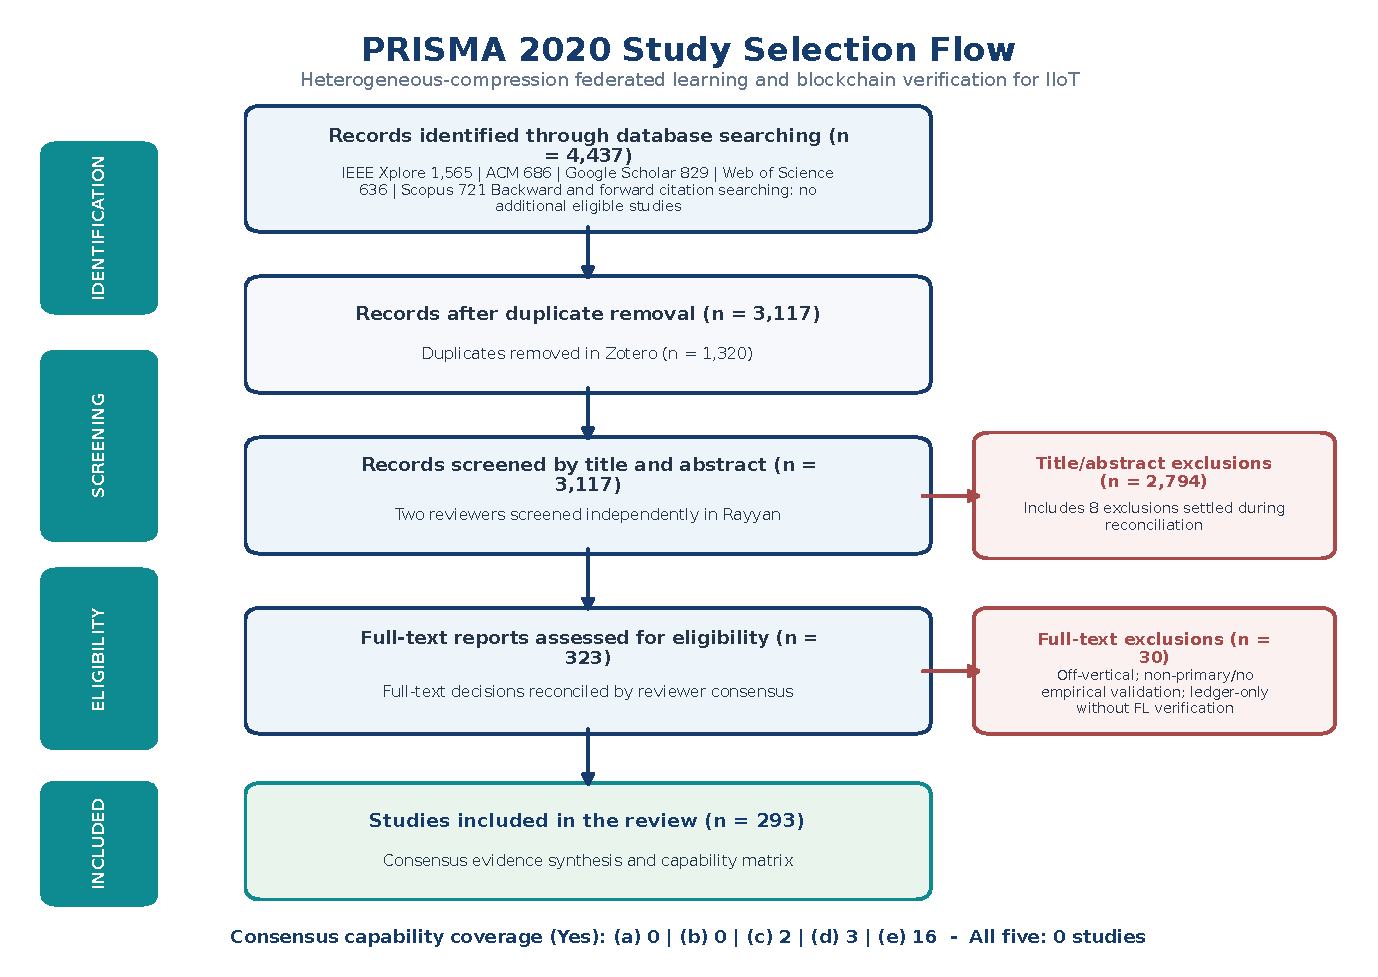
\includegraphics[width=0.9\textwidth]{figures/prisma_flow.pdf}
  \caption{PRISMA-style flow of study identification, screening, eligibility assessment, and inclusion. The title/abstract exclusion total includes eight exclusions settled during reviewer reconciliation.}
  \label{fig:prisma}
\end{figure*}

\section{Results}
\label{sec:results}

\subsection{Included evidence and capability coverage}
\label{subsec:coverage}

The final corpus comprised 293 studies. Table~\ref{tab:capability} reports the consensus capability scores. No included study received a Yes for live-resource-driven compression or convergence-guaranteed aggregation across mismatched models. Metadata-forgery threat models, constant-complexity verification, and heterogeneous multi-tier evaluation were present in a small subset of the corpus. No study satisfied all five capabilities, and none satisfied three or more or four or more capabilities according to the consensus summary.

\begin{table*}[!t]
\centering
\caption{Consensus coverage of the five review capabilities across 293 included studies.}
\label{tab:capability}
\begin{tabular}{p{0.47\textwidth}rrrr}
\toprule
\textbf{Capability} & \textbf{Yes} & \textbf{Partial} & \textbf{No} & \textbf{Yes (\%)} \\
\midrule
(a) Adaptive compression from live resource profiles & 0 & 1 & 292 & 0 \\
(b) Convergence-guaranteed aggregation across mismatched models & 0 & 8 & 285 & 0 \\
(c) Metadata-forgery threat model & 2 & 26 & 265 & 1 \\
(d) $O(1)$ on-chain verification & 3 & 21 & 269 & 1 \\
(e) Heterogeneous multi-tier evaluation & 16 & 23 & 254 & 5 \\
\bottomrule
\end{tabular}
\end{table*}

\subsection{RQ1: Compression-ratio selection}
\label{subsec:rq1}

The matrix records no Yes and one Partial judgment for compression ratios selected from live resource profiles. The extraction distinguishes fixed compression settings, preset device tiers, bandwidth-driven adaptation, and adaptation based on measured hardware state; these decision signals are not equivalent under capability (a). The current aggregate summary establishes the rarity of live-resource adaptation but does not provide verified counts for every compression-strategy subtype.

\subsection{RQ2: Aggregation under model-size mismatch}
\label{subsec:rq2}

No included study was coded Yes for convergence-guaranteed aggregation across mismatched model sizes; eight were coded Partial. This result identifies a need to make the aggregation assumptions explicit, including how parameter spaces are aligned, which client submodels participate in each round, and what convergence claim is established under the resulting mismatch. The review does not infer a formal guarantee from empirical convergence alone.

\subsection{RQ3: Integrity and metadata-forgery threats}
\label{subsec:rq3}

Two studies were coded Yes and 26 Partial for an explicit metadata-forgery threat model. The synthesis distinguishes forgery of update or participation metadata from broader Byzantine behavior, model poisoning, privacy leakage, and auditability. The extracted evidence records the stated contribution, limitations, and experimental context; interpretation of each mechanism should remain tied to the threat and verification claims actually reported in its source study.

\subsection{RQ4: On-chain verification and overhead}
\label{subsec:rq4}

Three studies were coded Yes and 21 Partial for $O(1)$ on-chain verification. The extracted matrix records gas, latency, memory, datasets, and testbed details when reported. The synthesis distinguishes asymptotic claims from measured costs and on-chain work from off-chain computation, setup, and communication overhead. The evidence does not support a single pooled overhead estimate without harmonized implementation and platform assumptions.

\subsection{RQ5: Unoccupied capability combinations}
\label{subsec:rq5}

The consensus matrix reports zero studies satisfying all five capabilities, zero satisfying four or more, and zero satisfying three or more. In addition, capabilities (a) and (b) each have zero Yes judgments across the included corpus. Within this review's search and eligibility scope, the evidence therefore points to a particularly sparse intersection between resource-profile-driven compression, principled aggregation under model mismatch, explicit metadata-forgery protection, lightweight verification, and evaluation on heterogeneous IIoT hardware. These are corpus-bounded findings, not claims that no relevant study exists outside the review.

\subsection{Full-text exclusions and agreement}
\label{subsec:agreement}

The 30 full-text exclusions were primarily classified as off-vertical settings (including vehicular, UAV, or metaverse contexts), non-primary or conceptual work without empirical validation, and ledger-only approaches without FL verification. The kappa summary reports $\kappa\approx0.61$ for title/abstract screening and $\kappa=0.615$ for full-text inclusion. The full-text paired-decision table contains 272 agreements on inclusion, 23 agreements on exclusion, and 24 disagreements among 319 paired decisions; the disagreements were resolved by consensus. Four additional full-text decisions lacked paired independent ratings.

\begin{figure}[!t]
  \centering
  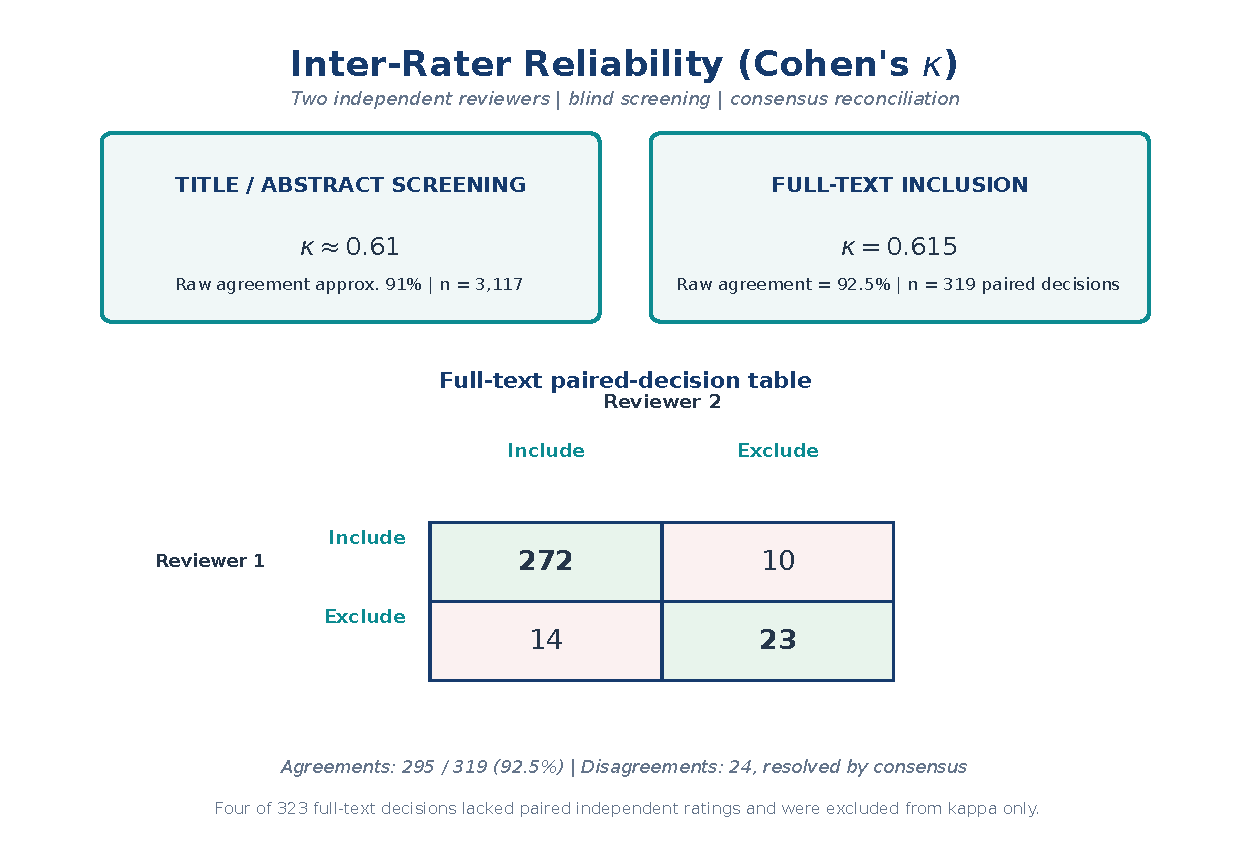
\includegraphics[width=\columnwidth]{figures/kappa_summary.pdf}
  \caption{Inter-rater reliability for title/abstract and full-text screening, including the paired-decision table for full-text inclusion.}
  \label{fig:kappa}
\end{figure}

\section{Discussion and Researcher Guidance}
\label{sec:discussion}

\subsection{Interpretation of the evidence}
\label{subsec:interpretation}

The strongest signal in the matrix is not simply that the five-capability intersection is empty: two foundational capabilities—live-resource-driven compression and convergence-guaranteed aggregation across mismatched models—received no Yes judgments. Researchers should therefore avoid treating compression, heterogeneity, robust aggregation, and blockchain as interchangeable labels. A study may address one dimension without operationalizing the others, and an empirical demonstration does not by itself establish a theoretical guarantee or an integrity threat model.

The capability counts also show a difference between partial and complete treatment. For metadata forgery and $O(1)$ verification, partial coverage is substantially more common than complete coverage. A useful reading of these partial scores requires case-level examples and the operational coding rubric, so readers can distinguish a narrowly implemented feature from evidence meeting the review's complete-capability threshold.

\subsection{Open research directions}
\label{subsec:agenda}

The review suggests the following directions for researchers:
\begin{itemize}
  \item \textbf{Measure resources and adapt explicitly:} report the device signals used to select compression, how often they are measured, and the policy mapping those signals to compression choices.
  \item \textbf{Analyze aggregation under structural mismatch:} state the relationship between client and server parameter spaces and establish convergence conditions for the actual aggregation procedure.
  \item \textbf{Specify integrity threats precisely:} separate metadata forgery from poisoning and generic Byzantine behavior, and evaluate detection against a stated adversary model.
  \item \textbf{Account for verification end to end:} define what is included in an $O(1)$ claim and report on-chain gas and latency together with off-chain computation, communication, and memory costs.
  \item \textbf{Evaluate across reproducible hardware tiers:} identify physical versus simulated devices, report hardware and software configurations, and distinguish system heterogeneity from non-IID data effects.
\end{itemize}

\subsection{Implications for review users}
\label{subsec:implications}

For researchers entering this area, the extraction matrix can be used as a comparison checklist rather than as a ranking of papers. For system designers, it highlights the need to justify device assumptions and to measure trade-offs across accuracy, convergence, compression, and verification overhead. For authors of future reviews and experiments, reporting exact search strategies, coding rules, hardware configurations, and threat models will improve reproducibility and make later evidence synthesis more reliable.

\section{Limitations}
\label{sec:limitations}

The findings are bounded by the selected sources, search period, eligibility criteria, and the completeness of the retrieved full texts. The exact database-specific queries, per-source search dates, and protocol publication start year must be verified against the saved search records before submission. The study-level synthesis depends on reviewer interpretation of reported methods; applying the more conservative score where ordinal ratings differed may reduce apparent capability coverage. Full-text kappa was calculated on 319 paired decisions rather than all 323 assessed full texts, and this distinction should be retained when reporting agreement. Finally, the matrix's capability counts should not be generalized beyond the included corpus or interpreted as evidence that a capability is impossible.

\section{Conclusion}
\label{sec:conclusion}

This systematic review synthesized 293 studies on heterogeneous-compression FL and blockchain-based verification in the context of resource-constrained IIoT. The consensus matrix found no included study coded Yes for live-resource-driven compression or convergence-guaranteed aggregation across mismatched models, and no study covered all five review capabilities together. The results provide a structured starting point for researchers to compare methods and identify under-addressed combinations. Stronger conclusions and reproducibility depend on retaining the bounded scope of these findings and completing the search-record checks noted in the methods before publication.

\section*{Acknowledgment}
This work was partly supported by IITP Innovative Human Resource Development for Local Intellectualization Program (MSIT) (IITP-2026-RS-2020-II201612, 34\%), IITP ITRC Program (MSIT) (IITP-2026-RS-2024-00438430, 33\%), NRF Basic Science Research Program (MOE) (2018R1A6A1A03024003, 33\%), and RISE (Regional Growth Innovation LAB) Program through Gyeongbuk RISE Center funded by MOE and Gyeongsangbuk-do, Republic of Korea (2026-rise-15-105).

\balance
\bibliographystyle{IEEEtran}
\bibliography{newref}
\end{document}
